% Template for PLoS
% Version 3.6 Aug 2022
%
% % % % % % % % % % % % % % % % % % % % % %
%
% -- IMPORTANT NOTE
%
% This template contains comments intended 
% to minimize problems and delays during our production 
% process. Please follow the template instructions
% whenever possible.
%
% % % % % % % % % % % % % % % % % % % % % % % 
%
% Once your paper is accepted for publication, 
% PLEASE REMOVE ALL TRACKED CHANGES in this file 
% and leave only the final text of your manuscript. 
% PLOS recommends the use of latexdiff to track changes during review, as this will help to maintain a clean tex file.
% Visit https://www.ctan.org/pkg/latexdiff?lang=en for info or contact us at latex@plos.org.
%
%
% There are no restrictions on package use within the LaTeX files except that no packages listed in the template may be deleted.
%
% Please do not include colors or graphics in the text.
%
% The manuscript LaTeX source should be contained within a single file (do not use \input, \externaldocument, or similar commands).
%
% % % % % % % % % % % % % % % % % % % % % % %
%
% -- FIGURES AND TABLES
%
% Please include tables/figure captions directly after the paragraph where they are first cited in the text.
%
% DO NOT INCLUDE GRAPHICS IN YOUR MANUSCRIPT
% - Figures should be uploaded separately from your manuscript file. 
% - Figures generated using LaTeX should be extracted and removed from the PDF before submission. 
% - Figures containing multiple panels/subfigures must be combined into one image file before submission.
% For figure citations, please use "Fig" instead of "Figure".
% See http://journals.plos.org/plosone/s/figures for PLOS figure guidelines.
%
% Tables should be cell-based and may not contain:
% - spacing/line breaks within cells to alter layout or alignment
% - do not nest tabular environments (no tabular environments within tabular environments)
% - no graphics or colored text (cell background color/shading OK)
% See http://journals.plos.org/plosone/s/tables for table guidelines.
%
% For tables that exceed the width of the text column, use the adjustwidth environment as illustrated in the example table in text below.
%
% % % % % % % % % % % % % % % % % % % % % % % %
%
% -- EQUATIONS, MATH SYMBOLS, SUBSCRIPTS, AND SUPERSCRIPTS
%
% IMPORTANT
% Below are a few tips to help format your equations and other special characters according to our specifications. For more tips to help reduce the possibility of formatting errors during conversion, please see our LaTeX guidelines at http://journals.plos.org/plosone/s/latex
%
% For inline equations, please be sure to include all portions of an equation in the math environment.  For example, x$^2$ is incorrect; this should be formatted as $x^2$ (or $\mathrm{x}^2$ if the romanized font is desired).
%
% Do not include text that is not math in the math environment. For example, CO2 should be written as CO\textsubscript{2} instead of CO$_2$.
%
% Please add line breaks to long display equations when possible in order to fit size of the column. 
%
% For inline equations, please do not include punctuation (commas, etc) within the math environment unless this is part of the equation.
%
% When adding superscript or subscripts outside of brackets/braces, please group using {}.  For example, change "[U(D,E,\gamma)]^2" to "{[U(D,E,\gamma)]}^2". 
%
% Do not use \cal for caligraphic font.  Instead, use \mathcal{}
%
% % % % % % % % % % % % % % % % % % % % % % % % 
%
% Please contact latex@plos.org with any questions.
%
% % % % % % % % % % % % % % % % % % % % % % % %

\documentclass[10pt,letterpaper]{article}
\usepackage[top=0.85in,left=2.75in,footskip=0.75in]{geometry}

% amsmath and amssymb packages, useful for mathematical formulas and symbols
\usepackage{amsmath,amssymb}

% Use adjustwidth environment to exceed column width (see example table in text)
\usepackage{changepage}

% textcomp package and marvosym package for additional characters
\usepackage{textcomp,marvosym}

% cite package, to clean up citations in the main text. Do not remove.
\usepackage{cite}

% Use nameref to cite supporting information files (see Supporting Information section for more info)
\usepackage{nameref,hyperref}

% line numbers
\usepackage[right]{lineno}

% ligatures disabled
\usepackage[nopatch=eqnum]{microtype}
\DisableLigatures[f]{encoding = *, family = * }

% color can be used to apply background shading to table cells only
\usepackage[table]{xcolor}

%% user-defined packages
\usepackage{ulem}
\usepackage{xspace}
\usepackage{hyperref}
\usepackage{enumitem}
\usepackage[export]{adjustbox}
\usepackage{subfig}
\usepackage{xltabular}
\usepackage{booktabs}
\usepackage{multirow}
\usepackage{tabularx}
\usepackage{tabularray}
\UseTblrLibrary{siunitx}
\usepackage{longtable}
\usepackage{csvsimple}
\usepackage{pdflscape}
\usepackage{geometry}

% create "+" rule type for thick vertical lines
\newcolumntype{+}{!{\vrule width 2pt}}

% create \thickcline for thick horizontal lines of variable length
\newlength\savedwidth
\newcommand\thickcline[1]{%
  \noalign{\global\savedwidth\arrayrulewidth\global\arrayrulewidth 2pt}%
  \cline{#1}%
  \noalign{\vskip\arrayrulewidth}%
  \noalign{\global\arrayrulewidth\savedwidth}%
}

% \thickhline command for thick horizontal lines that span the table
\newcommand\thickhline{\noalign{\global\savedwidth\arrayrulewidth\global\arrayrulewidth 2pt}%
\hline
\noalign{\global\arrayrulewidth\savedwidth}}


% Remove comment for double spacing
%\usepackage{setspace} 
%\doublespacing

% Text layout
\raggedright
\setlength{\parindent}{0.5cm}
\textwidth 5.25in 
\textheight 8.75in

% Bold the 'Figure #' in the caption and separate it from the title/caption with a period
% Captions will be left justified
\usepackage[aboveskip=1pt,labelfont=bf,labelsep=period,justification=raggedright,singlelinecheck=off]{caption}
\renewcommand{\figurename}{Fig}

% Use the PLoS provided BiBTeX style
\bibliographystyle{plos2015}

% Remove brackets from numbering in List of References
\makeatletter
\renewcommand{\@biblabel}[1]{\quad#1.}
\makeatother



% Header and Footer with logo
\usepackage{lastpage,fancyhdr,graphicx}
\usepackage{epstopdf}
%\pagestyle{myheadings}
\pagestyle{fancy}
\fancyhf{}
%\setlength{\headheight}{27.023pt}
%\lhead{\includegraphics[width=2.0in]{PLOS-submission.eps}}
\rfoot{\thepage/\pageref{LastPage}}
\renewcommand{\headrulewidth}{0pt}
\renewcommand{\footrule}{\hrule height 2pt \vspace{2mm}}
\fancyheadoffset[L]{2.25in}
\fancyfootoffset[L]{2.25in}
\lfoot{\today}

%% Include all macros below

\newcommand{\lorem}{{\bf LOREM}}
\newcommand{\ipsum}{{\bf IPSUM}}

%% END MACROS SECTION


\begin{document}
\vspace*{0.2in}

% Title must be 250 characters or less.
\begin{flushleft}
{\Large
\textbf\newline{Title of submission to PLOS journals} % Please use "sentence case" for title and headings (capitalize only the first word in a title (or heading), the first word in a subtitle (or subheading), and any proper nouns).
}
\newline
% Insert author names, affiliations and corresponding author email (do not include titles, positions, or degrees).
\\
Name1 Surname\textsuperscript{1,2\Yinyang},
Name2 Surname\textsuperscript{2\Yinyang},
Name3 Surname\textsuperscript{2,3\textcurrency},
Name4 Surname\textsuperscript{2},
Name5 Surname\textsuperscript{2\ddag},
Name6 Surname\textsuperscript{2\ddag},
Name7 Surname\textsuperscript{1,2,3*},
with the Lorem Ipsum Consortium\textsuperscript{\textpilcrow}
\\
\bigskip
\textbf{1} Affiliation Dept/Program/Center, Institution Name, City, State, Country
\\
\textbf{2} Affiliation Dept/Program/Center, Institution Name, City, State, Country
\\
\textbf{3} Affiliation Dept/Program/Center, Institution Name, City, State, Country
\\
\bigskip

% Insert additional author notes using the symbols described below. Insert symbol callouts after author names as necessary.
% 
% Remove or comment out the author notes below if they aren't used.
%
% Primary Equal Contribution Note
\Yinyang These authors contributed equally to this work.

% Additional Equal Contribution Note
% Also use this double-dagger symbol for special authorship notes, such as senior authorship.
\ddag These authors also contributed equally to this work.

% Current address notes
\textcurrency Current Address: Dept/Program/Center, Institution Name, City, State, Country % change symbol to "\textcurrency a" if more than one current address note
% \textcurrency b Insert second current address 
% \textcurrency c Insert third current address

% Deceased author note
\dag Deceased

% Group/Consortium Author Note
\textpilcrow Membership list can be found in the Acknowledgments section.

% Use the asterisk to denote corresponding authorship and provide email address in note below.
* correspondingauthor@institute.edu

\end{flushleft}
% Please keep the abstract below 300 words
\section*{Abstract}
this section will contain the abstract

% Please keep the Author Summary between 150 and 200 words
% Use first person. PLOS ONE authors please skip this step. 
% Author Summary not valid for PLOS ONE submissions.   
\section*{Author summary}
Refer to comments in the Latex template as this may not be necessary.

\linenumbers

\section*{Introduction}
this section will contain the introduction text

\section*{Materials and methods}

\subsection*{Cohort definition}
Both the original study by Shu et al.~\cite{shu2021predicting} and the subsequent replication and reproducibility study by 
Arafe et al.~\cite{Arafe2023.05.05.539590} selected patients with Parkinson's disease (PD) from the PPMI dataset and matched their 
age, sex, and H\&Y score from the first of two visits spanning approximately 36 months apart. For the first visit, each patient 
underwent an evaluation consisting of a clinical assessment and an MRI scan. They also had a follow-up clinical examination 3 years later. 
Patients were classified as 'progressive' if their H\&Y score at the follow-up visit exceeded the score from 3 years prior; otherwise, they 
were classified as 'stable'. Regarding inclusion criteria, Shu et al. created a cohort by limiting their selection to patients with MRI data 
from a Siemens Verio 3T MRI machine, incorporating restrictions on repetition time, echo time, inversion time, field of view, matrix size, 
and slice thickness. Their final cohort comprised 144 patients, equally distributed between progressive and stable subjects. 
On the other hand, rather than a single cohort, Arafe et al. constructed 5 cohorts, each consisting of 72 stable and 72 progressive subjects. One 
cohort aimed to replicate the Shu et al. cohort, while the other four were designed with different levels to assess the sensitivity of model predictions to 
the selection process.

Like Arafe et al. and Shu et al., as part of the selection process, we filtered the subjects in the PPMI database using the 
following inclusion criteria:
\begin{itemize}
  \item \textbf{C1}: patient has a diagnosis of idiopathic PD;
  \item \textbf{C2}: PPMI database contains records of at least 2 visits spaced approximately 3 years apart;
  \item \textbf{C3}: PPMI database contains a T1-weighted MRI from the first visit determined by C2;
  \item \textbf{C4}: PPMI database contains H\&Y scores for both visits. 
\end{itemize}

We assessed the impact of the MRI machine manufacturers and models on the collected image data and concluded that restrictions on these parameters could be relaxed. 
However, we ensured consistency across the selected subjects by standardizing the slice thickness and field strength across all MRI machines used. Consequently, our 7 
cohorts have been established according to the following additional criteria:

\begin{itemize}
  \item \textbf{C5}: all MRI machine manufacturers and models are permissable;
  \item \textbf{C6}: scanner restrictions: slice thickness = 1 mm and field strength = 3T;
\end{itemize}

After filtering the PPMI dataset for Criteria 1 to 6, visit pairs were formed for the remaining subjects while ensuring C2 and C3 remained true for each visit pair. 
During this phase, an additional restriction was imposed for the formation of Cohorts 1 to 6 such that a patient's functional state (also called PD state), which 
may be ``On" or ``Off", must be the same for both visits. The functional state of a patient, ``On" or ``Off", is determined by their PD medication status during clinical 
examinations. As the classification into progressive or stable groups depends on the stability of H\&Y scores over time, this restriction bolsters the comparability of 
these scores.

As the PPMI dataset is collected over an extended period of time and the protocol requires clinical evaluation in both ``On" and ``Off" functional states for every visit, many 
subjects have more than one visit pair and it is possible for a subject to be classified as both progressive and stable for different visit pairs. Therefore, after the 
creation of a cohort, validation checks were defined to ensure that any given subject was only included once, as either stable or progressive, in the resulting cohort. 

One of our objectives was to create the largest possible cohorts that adhered to the stated restrictions. Thus, although Cohorts 1, 3, 5, and 7 were created 
by matching patients from the progressive and stable classes on age, sex and H\&Y scores from the first visit, Cohorts 2, 4, and 6 used no matching filter.
This approach allowed for larger cohorts but necessitated the creation of demographics feature sets to evaluate the impact of this uneven distribution on the results. 
Cohorts 1 and 2 sampled visit pairs with PD state = "Off", Cohorts 5 and 6 sampled pairs with PD state = "On", and Cohorts 3 and 4 sampled visit pairs with 
either PD state = "Off" or PD state = "On" for both visits. Cohort 7 was defined without any restrictions on the PD state (see Fig~\ref{cohortCreationFlowchart}).

\begin{figure}[!ht]
  \centering
  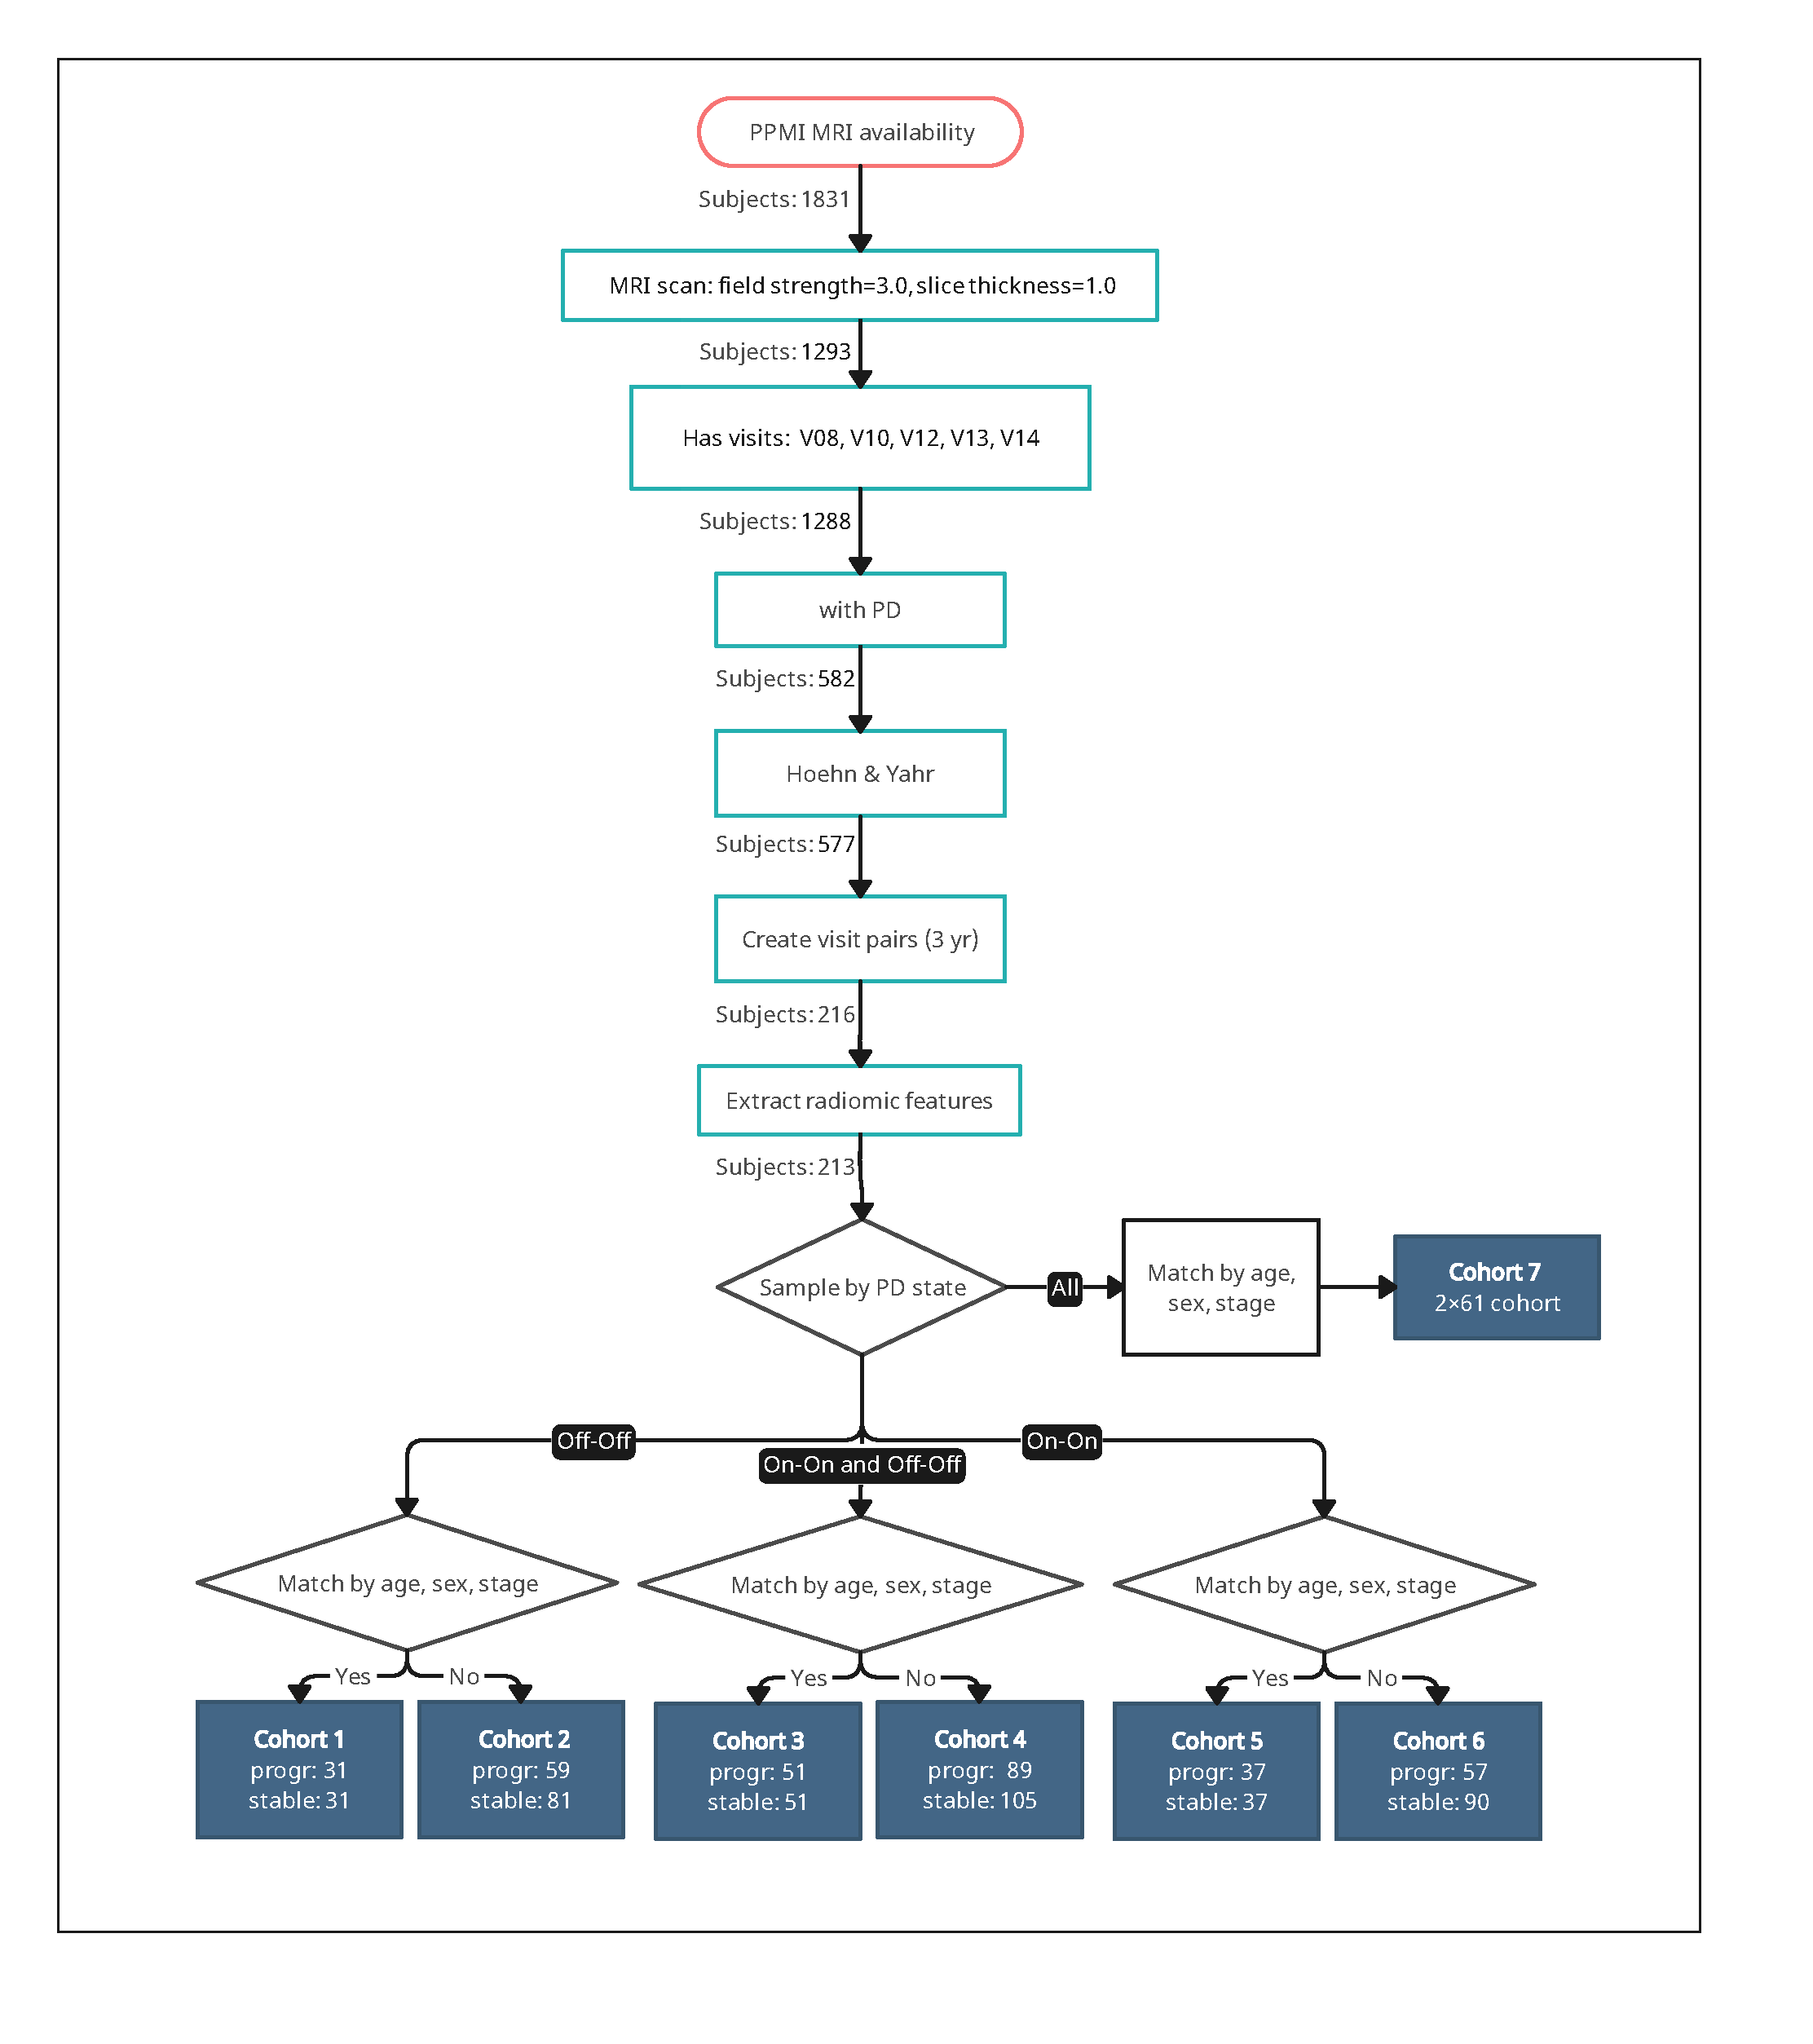
\includegraphics[width=\linewidth]{images/cohort_flowhart.pdf}
  \caption{{\bf Cohort construction} Process of filtering the PPMI dataset to construct 7 cohorts.}
  \label{cohortCreationFlowchart}
\end{figure}

\subsection*{Feature extraction}
We extracted nine sets of features for each cohort, labeled as F1 through F9. These feature sets are variations of Shu et al.'s original sets. Specifically, 
three sets are based on patient demographics, while the remaining six sets consist of radiomics-based features (See Fig~\ref{featureExtraction}).

\begin{figure}[!ht]
  \centering
  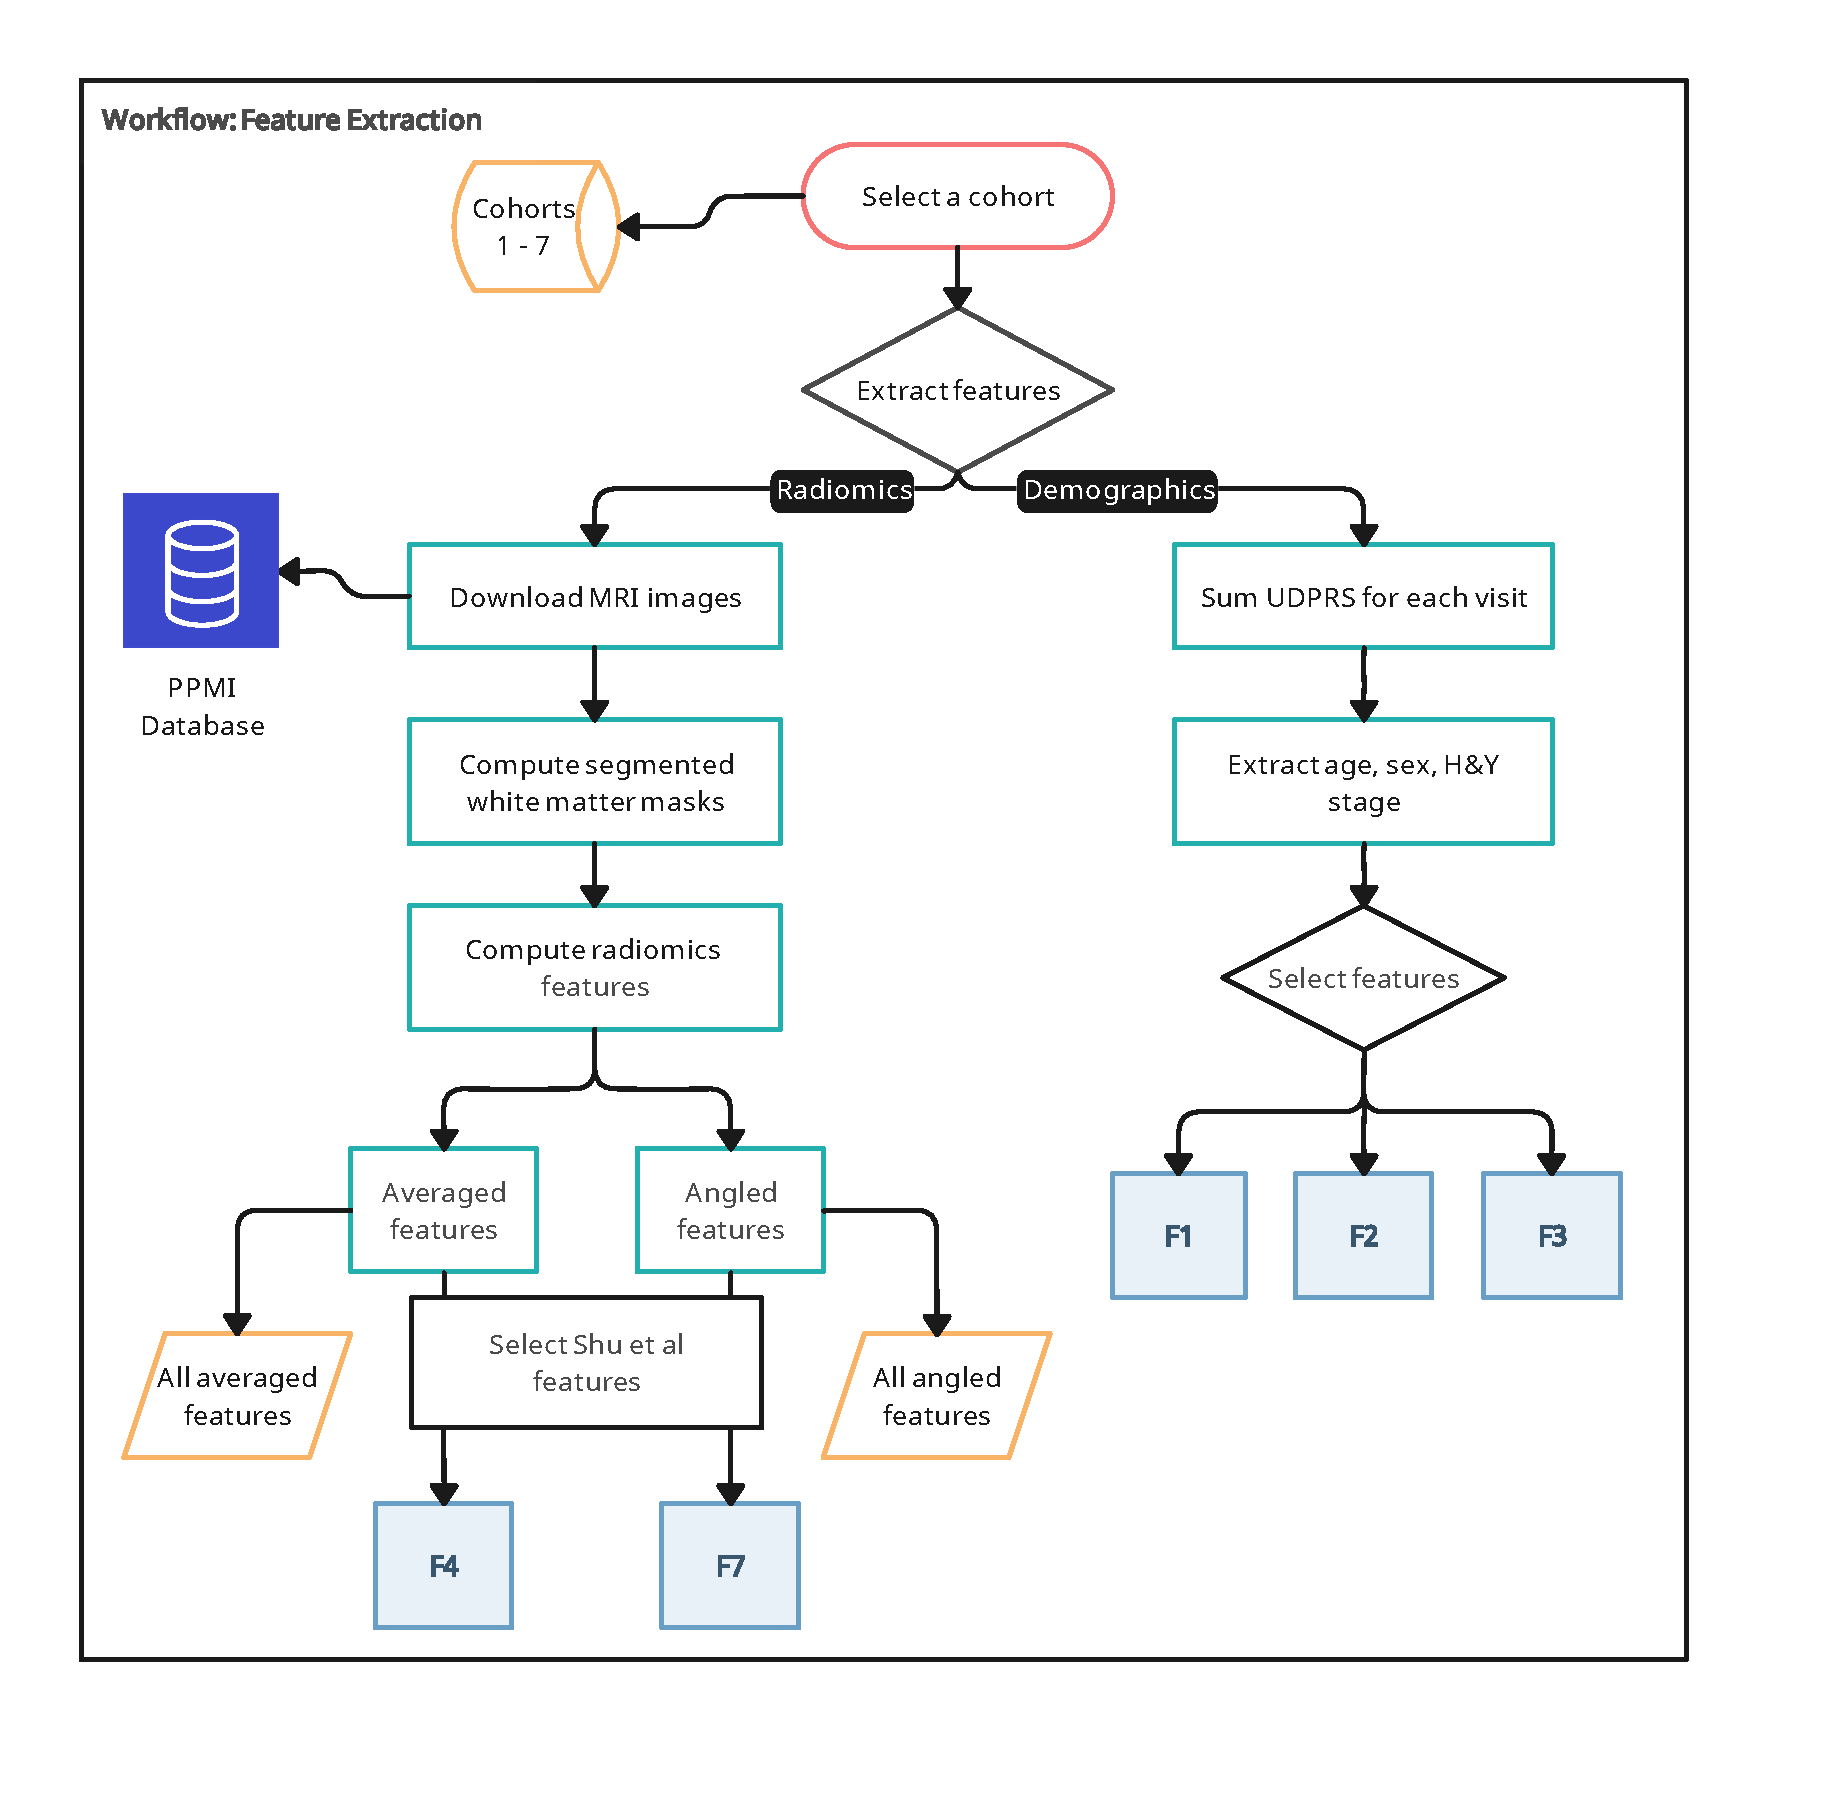
\includegraphics[width=\linewidth]{images/Workflow_feature_extraction.pdf}
  \caption{{\bf Feature Extraction} Extraction of the radiomic and demographic features.}
  \label{featureExtraction}
\end{figure}

\subsubsection*{Demographic features}
Three sets of demographic features were defined:

\begin{itemize}
    \item \textbf{F1}: age, sex, H\&Y score
    \item \textbf{F2}: age, sex, UPDRS total score
    \item \textbf{F3}: age, sex, H\&Y score, UPDRS total score
\end{itemize}


The selection of the age, sex, Unified Parkinson's Disease Rating Scale (UPDRS) total score, and the H\&Y score 
for the demographic features is due to the possibility that they may be contributing factors to whether a subject 
is classified as progressive or stable; meaning an imbalanced dataset with respect to these features may impact the results.  
The demographic features were taken from the first of the selected visits for each subject in the cohorts. While the age, sex, 
and H\&Y score were accessible in the study files from the PPMI database, the Unified Parkinson's Disease Rating Scale (UPDRS) scores 
are derived from a four part assessment of the motor and non-motor functions of a subject~\cite{goetz_tilley_shaftman_stebbins_fahn_martinez-martin_poewe_sampaio_stern_dodel_et_al._2008}. 
The scores from all four parts of the UPDRS assessment were summed to obtain the UPDRS total score.

\subsubsection*{Radiomic features}
The A.K. software (Artificial-Intelligent Radio-Genomics Kits; GE Healthcare, Chicago, IL, USA) used in Shu et al. is not publicly available. Therefore, we used PyRadiomics \cite{pyradiomics_2017}, an open-source Python package for the extraction of radiomics features. It is important to note that PyRadiomics is recognized in the IBSI (Image Biomarker Standardization Initiative) community \cite{Zwanenburg_2020}.

In Shu et al., the authors extracted a total of 378 features, including 42 histograms features, 10 Haralick features, 9 FormFactor features, 126 GLCM features, 180 GLRLM features, and 11 gray level region matrix features (GLZSM). From these 378 features, the authors used the maximum relevance minimum redundancy (mRMR) algorithm to extract the following top 7 features and train the model:
\begin{itemize}
    \item Feature 1: GLCMEntropy\_AllDirection\_offset1
    \item Feature 2: RunLengthNonuniformity\_angle45\_offset7
    \item Feature 3: Correlation\_angle45\_offset1
    \item Feature 4: HaralickCorrelation\_angle90\_offset4
    \item Feature 5: ShortRunEmphasis\_angle0\_offset7
    \item Feature 6: HaralickCorrelation\_AllDirection\_offset7
    \item Feature 7: Inertia\_AllDirection\_offset4
\end{itemize}

The first set of radiomic features, F4, refer to the set of PyRadiomics features that best match the 7 A.K software features from Shu et al., namely:

\begin{itemize}
    \item Feature 1: Joint Entropy
    \item Feature 2: Run Length Non Uniformity
    \item Feature 3 / Feature 4 / Feature 6: Correlation
    \item Feature 5: Short Run Low Gray Level Emphasis
    \item Feature 7: Contrast
\end{itemize}

For feature sets F5 and F6, we leveraged the entire set of relevant features extracted with PyRadiomics by applying two distinct feature selection techniques: Principal Component Analysis (PCA) for F5 and mRMR for F6. Further details regarding the parameters and implementation of these techniques will be provided in subsequent sections.

The mapping between A.K software and PyRadiomics features is not exact. Indeed, the A.K software, unlike PyRadiomics, provides every feature at a specific angle and offset. In PyRadiomics, for each feature class, the value of a feature is calculated for each angle separately, after which the mean of these values is returned. The exact definitions of these features are available in the PyRadiomics documentation (\url{https://pyradiomics.readthedocs.io/en/latest/features.html}) and in the supplementary material of~\cite{shu2021predicting}, Table S2. 

To address this issue, we developed an extended version of PyRadiomics that allows users to request features at specific angles and offsets. Using this extension, we were able to construct three additional feature sets. The first of three feature sets, F7, consists of the 7 features found in Shu et al. usign the same offset and angle. F8 and F9 utilize all features extracted at every angle and offset, applying both PCA and MRMR to derive a final set of features. Table ~\ref{table:feature_summary} summarizes the nine feature sets discussed.

\begin{table}[ht]
  \centering
  \captionof{table}{Summary of the nine feature sets.}
  \begin{tblr}{
    colspec={X[c,1] X[3,l]},
    column{1}={c},
    row{1}={c},
    hlines,
  }
    Feature Set & Summary. \\
    F1 & Patient demographics including age, sex, and H\&Y score. \\
    F2 & Patient demographics including age, sex, and UPDRS score. \\
    F3 & Patient demographics including age, sex, H\&Y score, and UPDRS score. \\
    F4 & PyRadiomics features aligned with Shu et al.'s A.K. Software features. \\
    F5 & PyRadiomics features with PCA feature selection. \\
    F6 & PyRadiomics features with MRMR feature selection. \\
    F7 & Angled PyRadiomics features aligned with Shu et al.'s A.K. Software features. \\
    F8 & Angled PyRadiomics features with PCA feature selection. \\
    F9 & Angled PyRadiomics features with MRMR feature selection. \\
  \end{tblr}
  \label{table:feature_summary}
\end{table}



\subsection*{MRI pre-processing}
\subsubsection*{Segmentation of T1-weighted images}
For feature sets \textbf{F4} to \textbf{F9}, we used the Segmentation module of Statistical Parametric Mapping (SPM; \url{https://www.fil.ion.ucl.ac.uk/spm/software/spm12} ~\cite{ashburner2012spm}) version 12 that was also the segmentation method used in Shu et al. We used SPM12's default parameters to get the tissue probability masks and build a WM binary mask for each patient. 


\subsubsection*{Quality control}

In Shu et al., two experienced neuro-radiologists used ITK-snap to manually edit WM segmentations. The modifications included (i) removal of non-brain tissue, brain stem and cerebellum and (ii) correcting segmentation errors in WM tissues. We used 3D Slicer v.5.0.3 to visualize and assess the quality of WM segmentations produced by SPM12. For each MRI scan, we reviewed the axial, coronal and sagittal slices. Data was excluded if it met at least one of the following criteria:

\begin{itemize}
    \item There is WM outside of the segmented WM mask;
    \item There is GM inside the segmented WM mask;
    \item The MRI has any common artifacts;
    \item The MRI has a low signal-to-noise (SNR) ratio.
\end{itemize}

\subsection*{Dimensionality reduction and feature selection}
For the demographics data, due to the limited number of features, we opted against applying any reduction techniques. As for the radiomic features, specifically F5, F6, F8 \& F9, we implemented two feature selection methods drawn from Shu et al.'s research: MRMR \cite{Ding_Peng} and PCA. 

We imported the MRMR library using the following GitHub repository (MRMR; \url{https://github.com/smazzanti/mrmr}) and used K=7 just as in Shu et al. Additionally, we imported the PCA library from scikit-learn. Our analysis involved testing PCA with different numbers of components (2, 3, 5, 7, 10) in a cross-validation pipeline. This comprehensive approach allowed us to explore the effectiveness of each technique in reducing dimensionality and selecting relevant features, thus enhancing the robustness of our analysis.

\subsection*{Models}
\subsubsection*{Image-based model}
To predict disease progression, Shu et al. trained a linear SVM based on the 7 top features extracted and selected from 
segmented WM masks of PD patients. The authors compared the SVM with three other machine learning methods, including 
Gaussian Naive Bayes (GNB), k-nearest neighbours (KNN), and decision tree (DT) classifiers. Since the methods of Shu et al. 
did not mention the name and values of the classification hyper-parameters that were optimized, we optimized the usual 
parameters for these classifiers using the ranges in Table~\ref{table:hyperParamTable}. We implemented the models using 
scikit-learn v1.1.3 and Python v3.10.4.

\begin{table}[h]
\centering
\begin{tabular}{|c|c|c|}
    \hline
    \textbf{Model} & \textbf{Hyper-parameter} & \textbf{Range} \\
    \hline
    SVM & 
    Regularization parameter & 0.1, 1, 10, 100, 1000 \\
    & Gamma & 1, 0.1, 0.01, 0.001, 0.0001 \\
    & Kernel type & Linear, Poly, RBF \\
    \hline
    Decision Tree & 
    Max depth of tree & 1, 2, 3, 4, 5, 8, 16, 32 \\
    & Max number of leaf nodes & 2, 3, 4 , … , 19 \\
    & Min samples to split node & 2, 3, 4, 5, 8, 12, 16, 20 \\
    \hline
    K-nearest neighbors & 
    Number of neighbors & 1, 2, 3, … , 30 \\
    & Power parameter & 1, 2 \\
    & Weight function & uniform, distance \\
    \hline
    Gaussian NB & 
    Distribution variance & \verb|np.logspace(0,-9, num=100)| \\
    \hline
\end{tabular}
\caption{Ranges used in hyper-parameter optimization.}
\label{table:hyperParamTable}
\end{table}

\subsubsection*{Demographics model}

For comparison and analysis purposes, we also trained linear SVM, GNB, KNN, and DT classifiers on the demographics 
feature sets F1 - F3 for each of the cohorts. As with the image based models, we implemented the models with 
scikit-learn v1.1.3 and Python v3.10.4. Furthermore, the hyperparameter optimization process was applied in the same fashion  
with the range of parameters listed in Table~\ref{table:hyperParamTable}.

\subsection*{Model evaluation}

\subsection*{Code availability}

\section*{Results}

\subsection*{Cohorts}
The demographics for Cohorts 1 to 7 are summarized in Table \ref{table:cohort_summary}. Cohorts 1 and 2 were sampled from the same set of visit pairs, comprising a 
maximum of 140 subjects with PD state = ``Off" for both visits. Cohort 2 randomly sampled one visit pair for each of the available subjects and 
distributed them to each class as evenly as possible. This resulted in 81 stable subjects and 59 progressive subjects. The mean age and standard deviation for the stable subjects 
is 60.5±9.6 and 62.0±9.4 for the progressive subjects. There are 32 females and 49 males in the stable group, 19 females and 40 males in the progressive group. 
Regarding H\&Y scores, 9 stable subjects have a score of 1, 71 a score of 2, and 1 has a score of 3. For the progressive subjects, 46 have an H\&Y 
score = 1 and 13 have an H\&Y score = 2. Cohort 1 is the smallest of the constructed cohorts with only 31 stable and 31 progressive subjects for a total of 62 
subjects. The stable and progressive groups are composed of 11 females and 20 males, and 12 females and 19 males respectively. The mean age and standard deviation for the stable 
subjects is 60.6±7.2 and 61.4±8.1 for the progressive subjects. There are 18 subjects with H\&Y score = 1 and 13 with score = 2 for both the stable and progressive 
groups.

Cohorts 3 and 4 sampled from a set of visit pairs for 194 subjects with either PD state = ``Off" or PD state =``On" for both visits. Cohort 3 has 102 subjects with 
51 subjects in each class. The stable group has 17 females and 34 males, whereas the progressive group has 19 females and 32 males. The mean age and standard deviation for the stable 
subjects and progressive subjects is 60.3±8.8 and 62.9±8.7 respectively. Both the stable and progressive groups have 25 subjects with H\&Y score = 1 and 26 subjects 
with H\&Y score = 2. Cohort 4 is the largest cohort and is composed of 105 stable subjects and 89 progressive subjects. The mean age and standard deviation for the 
stable and progressive groups are similar to one another at 62.1±9.7 and 62.7±10.0 respectively. Cohort 4 has 41 females and 64 males in the stable group, whereas the 
progressive group has 32 females and 57 males. The number of subjects in the stable group that have H\&Y score = 1 is 11, H\&Y score = 2 is 92, and H\&Y score = 3 is 2. 
The number of subjects in the progressive group that have an H\&Y score of 1, 2, or 3 are 63, 24, and 1 respectively.

Cohorts 5 and 6 sampled from the set of visit pairs defined for the 147 subjects with PD state = ``On" for both visits. Cohort 5 has 74 subjects evenly distributed into stable 
and progressive groups of 37 each. The stable group is composed of 11 females and 26 males, and the progressive group has 14 females and 23 males. The mean age and standard 
deviation for the stable group is 59.0±0.0 and 63.9±9.4 for the progressive group. There are 18 subjects in each group with H\&Y score = 1 and 19 subjects in each group 
with H\&Y score = 2. Cohort 6 has 90 stable subjects and 57 progressive subjects for a total of 147 subjects. The stable group is composed of 36 females and 54 males with a mean 
age and standard deviation of 63.0±9.9, and the progressive group has 21 females and 36 males with a mean age of 62.9±10.1. The stable group has 8 subjects with H\&Y score = 1, 82 subjects 
with H\&Y score = 2, and 0 subjects with H\&Y score = 3. In contrast, the progressive group has 38 subjects with H\&Y score = 1, 18 subjects with H\&Y score = 2, and 1 subjects with 
H\&Y score = 3. 

Cohort 7 is the only cohort that samples from a set of visit pairs for 213 subjects without any restrictions for the PD state of a patient. This cohort was developed as a 
reference cohort for comparison with those created by ~\cite{shu2021predicting} and ~\cite{Arafe2023.05.05.539590}. Cohort 7 has 61 stable and 61 progressive subjects for a total 
of 122 subjects. There are 23 females and 38 males in the stable group and 26 females and 35 males in the progressive group. The mean age and standard deviation is 60.1±9.2 and 
62.3±9.2 for the stable and progressive groups respectively. The stable and progressive groups each have 35 subjects with H\&Y score = 1 and 26 subjects with H\&Y score = 2. 

\newgeometry{top=1cm, bottom=2cm, left=3.5cm, right=1.5cm}
\begin{landscape}
  \captionof{table}{Summary of the seven constructed cohorts.}
  \begin{tblr}{
    colspec={X[l,1]*{14}{X[-0.6]}},
    column{1}={cmd=\bfseries},
    rowspec={*{7}{m{3em}}},
    row{1}={cmd=\bfseries},
    row{5}={cmd=\num[separate-uncertainty]},
    cell{5}{1}={guard},
    hlines,
    vlines={1,2,3,4,5,6,7,8}{solid},
  }
    & \SetCell[c=2]{c} Cohort 1 & & \SetCell[c=2]{c} Cohort 2 & & \SetCell[c=2]{c} Cohort 3 & & \SetCell[c=2]{c} Cohort 4 & & \SetCell[c=2]{c} Cohort 5 & & \SetCell[c=2]{c} Cohort 6  & & \SetCell[c=2]{c} Cohort 7 & \\
    & Stable & Progr & Stable & Progr & Stable & Progr & Stable & Progr & Stable & Progr & Stable & Progr & Stable & Progr \\
    Subjects, No. & 31 & 31 & 81 & 59 & 51 & 51 & 105 & 89 & 37 & 37 & 90 & 57 & 61 & 61 \\
    F/M No. & 11/20 & 12/19 & 32/49 & 19/40 & 17/34 & 19/32 & 41/64 & 32/57 & 11/26 & 14/23 & 36/54 & 21/36 & 23/38 & 26/35 \\
    \textbf{Age, mean SD} & 60.6 \pm 7.2 & 61.4 \pm 8.1 & 60.5 \pm 9.6 & 62.0 \pm 9.4 & 60.3 \pm 8.8 & 62.9 \pm 8.7 & 62.1 \pm 9.7 & 62.7 \pm 10.0 & 59.0 \pm 9.0 & 63.9 \pm 9.4 & 63.0 \pm 9.9 & 62.9 \pm 10.1 & 60.1 \pm 9.2 & 62.3 \pm 9.2 \\
    Hoehn \& Yahr Stage 1 (n) & 18 & 18 & 9 & 46 & 25 & 25 & 11 & 63 & 18 & 18 & 8 & 38 & 35 & 35 \\
    Hoehn \& Yahr Stage 2 (n) & 13 & 13 & 71 & 13 & 26 & 26 & 92 & 24 & 19 & 19 & 82 & 18 & 26 & 26 \\
    Hoehn \& Yahr Stage 3 (n) & 0 & 0 & 1 & 0 & 0 & 0 & 2 & 1 & 0 & 0 & 0 & 1 & 0 & 0 \\
  \end{tblr}
  \label{table:cohort_summary}
\end{landscape}
\restoregeometry

\newgeometry{top=1cm, bottom=2cm, left=2cm, right=2cm}
\begin{landscape}
  \begin{table}[!ht]
    \centering
    \caption{ROC AUC scores for Cohorts 1 to 7 for the feature sets F1 to F9}
    \label{table:results}
    \footnotesize
    \csvautobooktabular{./data/cohort_results2.csv}
  \end{table}
\end{landscape}
\restoregeometry

\subsection*{Model performance}

\subsection*{Feature sets}


\section*{Discussion}

This section discusses the findings.

\section*{Conclusion}

The conclusion is here. 

\section*{Supporting information}

% Include only the SI item label in the paragraph heading. Use the \nameref{label} command to cite SI items in the text.
\paragraph*{S1 Fig.}
\label{S1_Fig}
{\bf Bold the title sentence.} Add descriptive text after the title of the item (optional).

\section*{Acknowledgments}

\nolinenumbers

\bibliography{bib}

\end{document}

